% Options for packages loaded elsewhere
\PassOptionsToPackage{unicode}{hyperref}
\PassOptionsToPackage{hyphens}{url}
%
\documentclass[
]{book}
\usepackage{amsmath,amssymb}
\usepackage{lmodern}
\usepackage{iftex}
\ifPDFTeX
  \usepackage[T1]{fontenc}
  \usepackage[utf8]{inputenc}
  \usepackage{textcomp} % provide euro and other symbols
\else % if luatex or xetex
  \usepackage{unicode-math}
  \defaultfontfeatures{Scale=MatchLowercase}
  \defaultfontfeatures[\rmfamily]{Ligatures=TeX,Scale=1}
\fi
% Use upquote if available, for straight quotes in verbatim environments
\IfFileExists{upquote.sty}{\usepackage{upquote}}{}
\IfFileExists{microtype.sty}{% use microtype if available
  \usepackage[]{microtype}
  \UseMicrotypeSet[protrusion]{basicmath} % disable protrusion for tt fonts
}{}
\makeatletter
\@ifundefined{KOMAClassName}{% if non-KOMA class
  \IfFileExists{parskip.sty}{%
    \usepackage{parskip}
  }{% else
    \setlength{\parindent}{0pt}
    \setlength{\parskip}{6pt plus 2pt minus 1pt}}
}{% if KOMA class
  \KOMAoptions{parskip=half}}
\makeatother
\usepackage{xcolor}
\usepackage{color}
\usepackage{fancyvrb}
\newcommand{\VerbBar}{|}
\newcommand{\VERB}{\Verb[commandchars=\\\{\}]}
\DefineVerbatimEnvironment{Highlighting}{Verbatim}{commandchars=\\\{\}}
% Add ',fontsize=\small' for more characters per line
\usepackage{framed}
\definecolor{shadecolor}{RGB}{248,248,248}
\newenvironment{Shaded}{\begin{snugshade}}{\end{snugshade}}
\newcommand{\AlertTok}[1]{\textcolor[rgb]{0.94,0.16,0.16}{#1}}
\newcommand{\AnnotationTok}[1]{\textcolor[rgb]{0.56,0.35,0.01}{\textbf{\textit{#1}}}}
\newcommand{\AttributeTok}[1]{\textcolor[rgb]{0.77,0.63,0.00}{#1}}
\newcommand{\BaseNTok}[1]{\textcolor[rgb]{0.00,0.00,0.81}{#1}}
\newcommand{\BuiltInTok}[1]{#1}
\newcommand{\CharTok}[1]{\textcolor[rgb]{0.31,0.60,0.02}{#1}}
\newcommand{\CommentTok}[1]{\textcolor[rgb]{0.56,0.35,0.01}{\textit{#1}}}
\newcommand{\CommentVarTok}[1]{\textcolor[rgb]{0.56,0.35,0.01}{\textbf{\textit{#1}}}}
\newcommand{\ConstantTok}[1]{\textcolor[rgb]{0.00,0.00,0.00}{#1}}
\newcommand{\ControlFlowTok}[1]{\textcolor[rgb]{0.13,0.29,0.53}{\textbf{#1}}}
\newcommand{\DataTypeTok}[1]{\textcolor[rgb]{0.13,0.29,0.53}{#1}}
\newcommand{\DecValTok}[1]{\textcolor[rgb]{0.00,0.00,0.81}{#1}}
\newcommand{\DocumentationTok}[1]{\textcolor[rgb]{0.56,0.35,0.01}{\textbf{\textit{#1}}}}
\newcommand{\ErrorTok}[1]{\textcolor[rgb]{0.64,0.00,0.00}{\textbf{#1}}}
\newcommand{\ExtensionTok}[1]{#1}
\newcommand{\FloatTok}[1]{\textcolor[rgb]{0.00,0.00,0.81}{#1}}
\newcommand{\FunctionTok}[1]{\textcolor[rgb]{0.00,0.00,0.00}{#1}}
\newcommand{\ImportTok}[1]{#1}
\newcommand{\InformationTok}[1]{\textcolor[rgb]{0.56,0.35,0.01}{\textbf{\textit{#1}}}}
\newcommand{\KeywordTok}[1]{\textcolor[rgb]{0.13,0.29,0.53}{\textbf{#1}}}
\newcommand{\NormalTok}[1]{#1}
\newcommand{\OperatorTok}[1]{\textcolor[rgb]{0.81,0.36,0.00}{\textbf{#1}}}
\newcommand{\OtherTok}[1]{\textcolor[rgb]{0.56,0.35,0.01}{#1}}
\newcommand{\PreprocessorTok}[1]{\textcolor[rgb]{0.56,0.35,0.01}{\textit{#1}}}
\newcommand{\RegionMarkerTok}[1]{#1}
\newcommand{\SpecialCharTok}[1]{\textcolor[rgb]{0.00,0.00,0.00}{#1}}
\newcommand{\SpecialStringTok}[1]{\textcolor[rgb]{0.31,0.60,0.02}{#1}}
\newcommand{\StringTok}[1]{\textcolor[rgb]{0.31,0.60,0.02}{#1}}
\newcommand{\VariableTok}[1]{\textcolor[rgb]{0.00,0.00,0.00}{#1}}
\newcommand{\VerbatimStringTok}[1]{\textcolor[rgb]{0.31,0.60,0.02}{#1}}
\newcommand{\WarningTok}[1]{\textcolor[rgb]{0.56,0.35,0.01}{\textbf{\textit{#1}}}}
\usepackage{longtable,booktabs,array}
\usepackage{calc} % for calculating minipage widths
% Correct order of tables after \paragraph or \subparagraph
\usepackage{etoolbox}
\makeatletter
\patchcmd\longtable{\par}{\if@noskipsec\mbox{}\fi\par}{}{}
\makeatother
% Allow footnotes in longtable head/foot
\IfFileExists{footnotehyper.sty}{\usepackage{footnotehyper}}{\usepackage{footnote}}
\makesavenoteenv{longtable}
\usepackage{graphicx}
\makeatletter
\def\maxwidth{\ifdim\Gin@nat@width>\linewidth\linewidth\else\Gin@nat@width\fi}
\def\maxheight{\ifdim\Gin@nat@height>\textheight\textheight\else\Gin@nat@height\fi}
\makeatother
% Scale images if necessary, so that they will not overflow the page
% margins by default, and it is still possible to overwrite the defaults
% using explicit options in \includegraphics[width, height, ...]{}
\setkeys{Gin}{width=\maxwidth,height=\maxheight,keepaspectratio}
% Set default figure placement to htbp
\makeatletter
\def\fps@figure{htbp}
\makeatother
\setlength{\emergencystretch}{3em} % prevent overfull lines
\providecommand{\tightlist}{%
  \setlength{\itemsep}{0pt}\setlength{\parskip}{0pt}}
\setcounter{secnumdepth}{5}
\usepackage{booktabs}
\ifLuaTeX
  \usepackage{selnolig}  % disable illegal ligatures
\fi
\usepackage[]{natbib}
\bibliographystyle{apalike}
\IfFileExists{bookmark.sty}{\usepackage{bookmark}}{\usepackage{hyperref}}
\IfFileExists{xurl.sty}{\usepackage{xurl}}{} % add URL line breaks if available
\urlstyle{same} % disable monospaced font for URLs
\hypersetup{
  pdftitle={Data Science for Social Scientists},
  pdfauthor={Daniel E. Ehrlich, IPUMS, University of Minnesota; Anna Tremblay, Dept of Soc, Anth, \& CJ, Clemson University},
  hidelinks,
  pdfcreator={LaTeX via pandoc}}

\title{Data Science for Social Scientists}
\usepackage{etoolbox}
\makeatletter
\providecommand{\subtitle}[1]{% add subtitle to \maketitle
  \apptocmd{\@title}{\par {\large #1 \par}}{}{}
}
\makeatother
\subtitle{An applied course using IPUMS data}
\author{Daniel E. Ehrlich, \href{https://international.ipums.org/international/}{IPUMS, University of Minnesota} \and Anna Tremblay, \href{https://www.clemson.edu/cbshs/departments/sacj/degrees/anthropology.html}{Dept of Soc, Anth, \& CJ, Clemson University}}
\date{2022-09-07}

\begin{document}
\maketitle

{
\setcounter{tocdepth}{1}
\tableofcontents
}
\hypertarget{preface}{%
\chapter*{Preface}\label{preface}}
\addcontentsline{toc}{chapter}{Preface}

An open-source book using open-source tools and nearly open-source data.

\hypertarget{what-is-ipums}{%
\section*{What is IPUMS}\label{what-is-ipums}}
\addcontentsline{toc}{section}{What is IPUMS}

IPUMS started as a project to digitize the historical records of the US census. It has expanded to include \href{https://www.ipums.org/}{9 data collections}, which are united in their methods and principles of making soial science research easier. IPUMS data consists of individual-level census and survey data from more than 100 countries around the world. Notably:

\begin{itemize}
\tightlist
\item
  IPUMS \textbf{harmonizes} these data, ensuring consistently coded values across time and space.
\item
  IPUMS provides harmonized \textbf{GIS Shapefiles} for most census and survey data
\item
  IPUMS provides extensive \textbf{metadata}, including

  \begin{itemize}
  \tightlist
  \item
    Original questionnaire text
  \item
    Alerts about notable changes in variable definition, universe, or coding
  \end{itemize}
\end{itemize}

IPUMS data is free to use for education and research purposes. Researchers just need to register with an \textbf{email address} and brief project description. Nothing too formal - we're just trying to understand what kinds of questions researchers are interested in. For educators, we have additional resources to set up \href{}{classroom accounts}, making it easy to get your students registered and share IPUMS data with them.

\hypertarget{why-make-this-course}{%
\section*{Why make this course}\label{why-make-this-course}}
\addcontentsline{toc}{section}{Why make this course}

While we (DEE) may be slightly biased, we think IPUms is a fantastic resource for \textbf{Education} and \textbf{Research}. Real-world example datasets provide the bulk of the content for this course, providing an \textbf{applied context} we hope students (and instructors) will find engaging. We also know meany instructors may be teaching across multiple disciplines, in large departments, or be the only ``data person'' at their instutition. We think IPUMS data will be useful to virtually any social science field. We provide some example lessons, and encourage instructors to develop their own, using our \texttt{template}, to tailor this course to their subject or interest.

\hypertarget{course-description}{%
\chapter*{Course Description}\label{course-description}}
\addcontentsline{toc}{chapter}{Course Description}

This course is broken down into 3, 5-week units. Unit 1 focuses on familiarizing yourself with R and the IPUMS dataset. In Unit 2, each week will showcase a method/analysis using preselected variables. In class, students will walk through a given problem set and produce a lab report by the end of class. In Unit 3, students will work towards answering a research question that they pose, creating a research paper with literature review, data analysis, conclusion, and data outputs.

\hypertarget{course-aims}{%
\section*{Course Aims}\label{course-aims}}
\addcontentsline{toc}{section}{Course Aims}

Provide students with relevant, hands on, methodological training in data literacy and visualization.

\hypertarget{learning-outcomes}{%
\section*{LEARNING OUTCOMES}\label{learning-outcomes}}
\addcontentsline{toc}{section}{LEARNING OUTCOMES}

LEARNING OUTCOMES:

\begin{itemize}
\item
  Understand the depth of the IPUMS database and the variables it has to\\
  offer
\item
  Compose R code to analyze the IPUMS data
\item
  Produce visually pleasing data outputs in R
\item
  Synthesize the information in a written report
\item
  Present the analysis in a poster format for other students
\end{itemize}

\hypertarget{guiding-principles}{%
\section*{Guiding Principles}\label{guiding-principles}}
\addcontentsline{toc}{section}{Guiding Principles}

\begin{itemize}
\tightlist
\item
  phenomenon-based learning

  \begin{itemize}
  \tightlist
  \item
    try to start the class with a \textbf{question} or \textbf{problem}
  \item
    \emph{why} does the data look the way it does
  \item
    structure class so students work towards solving the problem
  \end{itemize}
\item
  RELEVANT examples

  \begin{itemize}
  \tightlist
  \item
    try to touch on 2 or more disciplines (eg, economics, demography)
  \end{itemize}
\end{itemize}

\hypertarget{syllabus}{%
\chapter*{Syllabus}\label{syllabus}}
\addcontentsline{toc}{chapter}{Syllabus}

This syllabus is initially envisioned as 3 5-week sections. However, compilation and content are intended to be modular with templates for instructors to include their own specialties.

The basic structure of this course is:

Unit 1 (Weeks 1-5): Understanding and Testing Data

\begin{itemize}
\item
  Students use simple datasets

  \begin{itemize}
  \item
    Data provided by the course/instructor
  \item
    simplified data to illustrate trends

    \begin{itemize}
    \tightlist
    \item
      EG: Age distributions ; Age by Sex
    \item
      potential usecase for synthesized data
    \end{itemize}
  \end{itemize}
\end{itemize}

Unit 2 (Weeks 6-10): Finding Data and Asking Questions
* Students begin to analyze more complex (IPUMS) datasets
+ Data provided by course/instructor
+ IPUMS data testing/demonstrating real world effects
+ EG: SEX \textasciitilde{} EDUATTAIN ; Sex by eduattain by some SES indicators
+ Students are given a medium/large set of IPUMS variables
+ Students learn to perform exploratory analysis to guide hypotheses
* Students learn to navigate IPUMS website
+ Students learn to develop a hypothesis and find relevant data

Unit 3 (Weeks 11-15): Discussing Data and Student Research
* Students develop a research question to be answered with IPUMS data
* Students are encouraged to fit it to their interests/major/disciplie
* Course time should be devoted to individual/small-group research
* Instructor/class present on recent research
* Instructor models constructive / scholarly criticism
* Encourage students to critque published work - responsibly

\hypertarget{unit-1-5-weeks-understanding-and-testing-data}{%
\subsection*{Unit 1 (5 weeks) Understanding and Testing Data}\label{unit-1-5-weeks-understanding-and-testing-data}}
\addcontentsline{toc}{subsection}{Unit 1 (5 weeks) Understanding and Testing Data}

\hypertarget{week-1-intro-to-r-data-types-data-structures}{%
\subsubsection*{Week 1: Intro to R, data types, data structures}\label{week-1-intro-to-r-data-types-data-structures}}
\addcontentsline{toc}{subsubsection}{Week 1: Intro to R, data types, data structures}

\hypertarget{week-2-plotting-data-distributions}{%
\subsubsection*{Week 2: Plotting Data, Distributions}\label{week-2-plotting-data-distributions}}
\addcontentsline{toc}{subsubsection}{Week 2: Plotting Data, Distributions}

\hypertarget{week-3-statisitcal-testing-of-simple-data-sets}{%
\subsubsection*{Week 3: Statisitcal testing of simple data sets}\label{week-3-statisitcal-testing-of-simple-data-sets}}
\addcontentsline{toc}{subsubsection}{Week 3: Statisitcal testing of simple data sets}

\hypertarget{week-4-correlation-and-relationships-of-simple-data-sets}{%
\subsubsection*{Week 4: Correlation and Relationships of simple data sets}\label{week-4-correlation-and-relationships-of-simple-data-sets}}
\addcontentsline{toc}{subsubsection}{Week 4: Correlation and Relationships of simple data sets}

\hypertarget{week-5-tbd}{%
\subsubsection*{Week 5: (TBD)}\label{week-5-tbd}}
\addcontentsline{toc}{subsubsection}{Week 5: (TBD)}

\hypertarget{addl-details}{%
\subsubsection*{Addl Details}\label{addl-details}}
\addcontentsline{toc}{subsubsection}{Addl Details}

Intro to data/ simple analysis

Students will be able to:

Technical:

\begin{itemize}
\tightlist
\item
  Download R and RStudio
\item
  Read data into R and
\item
  Write (save) data out of R.
\item
  Summarize data visually

  \begin{itemize}
  \tightlist
  \item
    Using base R
  \item
    Using ggplot (tidyverse)
  \end{itemize}
\item
  Summarize data tabularly

  \begin{itemize}
  \tightlist
  \item
    Using base R
  \item
    Using gttable / tidyverse
  \end{itemize}
\item
  Formally state and test assumptions of data

  \begin{itemize}
  \tightlist
  \item
    \emph{EG:} t-test, anova, (maybe) correlations
  \end{itemize}
\end{itemize}

Conceptual:

\begin{itemize}
\tightlist
\item
  Understand main types of data

  \begin{itemize}
  \tightlist
  \item
    \emph{EG:} logical, numeric, character, etc
  \item
    R specic vs general terms
  \end{itemize}
\item
  Recgonize various data distributions

  \begin{itemize}
  \tightlist
  \item
    \emph{EG:} normal, poisson, etc
  \end{itemize}
\item
  Know which types statistical tests are appropriate for a given set of data.
\end{itemize}

\hypertarget{unit-2-finding-data-and-asking-questions-using-ipums-data}{%
\subsection*{Unit 2 Finding Data and Asking Questions (Using IPUMS Data)}\label{unit-2-finding-data-and-asking-questions-using-ipums-data}}
\addcontentsline{toc}{subsection}{Unit 2 Finding Data and Asking Questions (Using IPUMS Data)}

\hypertarget{week-6-exploratory-analysis}{%
\subsubsection*{Week 6 Exploratory analysis}\label{week-6-exploratory-analysis}}
\addcontentsline{toc}{subsubsection}{Week 6 Exploratory analysis}

\hypertarget{week-7-hypothesis-testing}{%
\subsubsection*{Week 7 Hypothesis Testing}\label{week-7-hypothesis-testing}}
\addcontentsline{toc}{subsubsection}{Week 7 Hypothesis Testing}

\hypertarget{week-8-statistical-inference}{%
\subsubsection*{Week 8 Statistical Inference}\label{week-8-statistical-inference}}
\addcontentsline{toc}{subsubsection}{Week 8 Statistical Inference}

\hypertarget{week-9-tbd}{%
\subsubsection*{Week 9 (TBD)}\label{week-9-tbd}}
\addcontentsline{toc}{subsubsection}{Week 9 (TBD)}

\hypertarget{week-10-tbd}{%
\subsubsection*{Week 10 (TBD)}\label{week-10-tbd}}
\addcontentsline{toc}{subsubsection}{Week 10 (TBD)}

\hypertarget{addl-details-1}{%
\subsubsection{Addl Details}\label{addl-details-1}}

Here we demonstrate two \textbf{different} approaches to conducting research. Students become familar writing up short lab reports detailing their findings. For unit \ref{expo}, we/instructor provides students with simple datasets from IPUMS (or other real-world data). Students will learn exploratory data analysis techniques and how to create lab reports to summarize key findings.

For unit \ref{hypo}, students will learn to develop their own simple research questions or social-science hypotheses. They will seek out data to answer these questions, learning to navigate \href{https://ipums.org}{ipums.org}, and create \textbf{data extracts}, as well as hypothesis-testing statistical methods. Again, lab reports to summarize findings.

\hypertarget{expo}{%
\paragraph{Exploratory Analysis}\label{expo}}

If you've just collected a survey, or other raw data, you may not know what you're looking for. This is perfectly ok but goes against \emph{the scientific method} most people learned in grade school (More on that to follow(\textbf{\emph{include\_link}})).

This unit begins by presenting data/distributions and asking students to begin interpreting the data . visual exploration is encouraged and basic of data manipulation are taught
* \emph{EG:} how to subset data, how to reshape data, how to recode data, how to convert from one \texttt{data\ type} to another.

Example lab exercise:

Students given a data set (xls, csv, etc)
* load data, perform manipulations, basic summaries
+ cross tabs
+ group means by a covariate
* inspect data visually
+ \emph{DESCRIBE} the distribution - is it normal? significant?
* \emph{FIND} aquestion in the spread of the data
+ how can you test this (maybe small group work)
* write up/ present results
+ think on confounding factors / biases

\hypertarget{hypo}{%
\paragraph{Hypotethsis Driven}\label{hypo}}

If, on the other hand you have an a pre-exisiting idea you want to test. We can follow the traditional \emph{scientific method}. With a question in mind, the first question is: where to look. What better place than \href{https://ipums.org}{IPUMS}!

Begin introducing navigation of web resources - mainly IPUMS international

Students should become comfortable working through lab exercises:
* Define a question (or be presented with one)
* Download variables from IPUMS (course downloads possible)
* Perform a basic analysis (discussed in Unit 1)
* Generate a \textbf{visual argument} for your analysis
+ Include explanation/interpretation/reflection on the question at hand, and the data used
+ Any obvious biases
+ Any obvious confounding factors

\hypertarget{unit-3-discussing-data-and-student-research}{%
\subsection*{Unit 3 Discussing Data and Student Research}\label{unit-3-discussing-data-and-student-research}}
\addcontentsline{toc}{subsection}{Unit 3 Discussing Data and Student Research}

\hypertarget{week-11-students-develop-research-question}{%
\subsubsection*{Week 11: Students develop research Question}\label{week-11-students-develop-research-question}}
\addcontentsline{toc}{subsubsection}{Week 11: Students develop research Question}

\hypertarget{week-12-students-find-relevant-variables-from-ipums}{%
\subsubsection*{Week 12: Students find relevant variables from IPUMS}\label{week-12-students-find-relevant-variables-from-ipums}}
\addcontentsline{toc}{subsubsection}{Week 12: Students find relevant variables from IPUMS}

\hypertarget{week-13-students-test-and-evaluate-results}{%
\subsubsection*{Week 13: Students test and evaluate results}\label{week-13-students-test-and-evaluate-results}}
\addcontentsline{toc}{subsubsection}{Week 13: Students test and evaluate results}

\hypertarget{week-14-students-prepare-presentations-of-results}{%
\subsubsection*{Week 14: Students prepare presentations of results}\label{week-14-students-prepare-presentations-of-results}}
\addcontentsline{toc}{subsubsection}{Week 14: Students prepare presentations of results}

\hypertarget{week-15-students-present-work-slides-poster-podium-etc}{%
\subsubsection*{Week 15: Students present work (slides, poster, podium, etc)}\label{week-15-students-present-work-slides-poster-podium-etc}}
\addcontentsline{toc}{subsubsection}{Week 15: Students present work (slides, poster, podium, etc)}

\hypertarget{addl-details-2}{%
\subsubsection{Addl Details}\label{addl-details-2}}

Students will select their own research question that can be answered with the IPUMS data set and will spend five weeks producing a research paper complete with data analysis, visualization, and interpretation.

In this section we encourage the instructor to provide ample time for independent student/small-group research. Some class time should be devoted to modelling healthy discussion and critique of methods.

We provide some examples here but encourage instructors (or students) to bring in recent journal/popular articles that do (or do not) apply data science methods well.

\hypertarget{dev-notes}{%
\chapter*{DEV NOTES}\label{dev-notes}}
\addcontentsline{toc}{chapter}{DEV NOTES}

\hypertarget{to-do}{%
\paragraph*{TO DO}\label{to-do}}
\addcontentsline{toc}{paragraph}{TO DO}

\begin{itemize}
\item
  Make chapter 1 chapter 2
\item
  Anna Adds chapter con data science intro exclusive of R/IPUMS
\item
  discuss style

  \begin{itemize}
  \tightlist
  \item
    key terms section for each chapter?
  \item
    key terms in \textbf{bold}
  \item
    italics for \emph{emphasis}
  \item
    are we pro-hyphens, or are they pedantic?
  \end{itemize}
\end{itemize}

\hypertarget{misc-ideas}{%
\paragraph*{MISC IDEAS}\label{misc-ideas}}
\addcontentsline{toc}{paragraph}{MISC IDEAS}

\begin{itemize}
\tightlist
\item
  Application forward
\item
  Present research/ analysis/results FIRST, then explain the mathematical principals behind it
\item
  daily/weekly ``i'm stuck on\ldots{}''

  \begin{itemize}
  \tightlist
  \item
    Students send in questions (night before class) and instructor spends 10-15 mins talking through (or collaboratively working through with class) solutions
  \item
    Alternatively, once a month maybe a longer class covering ``common problems asked this month''
    daily/weekly ``recent research''
  \end{itemize}
\item
  pick out a recent article with good visualization (or bad) and spend 5-10 mins discussing what makes it good (or bad)

  \begin{itemize}
  \tightlist
  \item
    Encourage students to find articles for extra credit
  \end{itemize}
\end{itemize}

\hypertarget{documentation}{%
\paragraph*{Documentation}\label{documentation}}
\addcontentsline{toc}{paragraph}{Documentation}

This function grabs any packages in your project and adds them to a local list that can be referenced using \texttt{R-pacakgename}
* \textbf{NOTE} in practice, that needs to be wrapped in markdown syntax, eg:
\texttt{{[}@R-bookdown{]}}
* See help files for more info - might be able to create/add a \texttt{citation} file

\hypertarget{unit1}{%
\chapter{Unit 1: The Basics}\label{unit1}}

\hypertarget{week-1-intro-to-r-data-types-data-structures-1}{%
\section{Week 1: Intro to R, data types, data structures}\label{week-1-intro-to-r-data-types-data-structures-1}}

\hypertarget{week-2-plotting-data-distributions-1}{%
\section{Week 2: Plotting Data, Distributions}\label{week-2-plotting-data-distributions-1}}

\hypertarget{normal-distributions}{%
\subsection{Normal Distributions}\label{normal-distributions}}

First we'll generate a normal distribution with the \texttt{rnorm()} function. This takes 3 arguments: \texttt{n,\ mean,\ sd}, which you can see filled in below. While we could print out a list of all these values, it's not easy to \emph{understand} a list of numbers

\begin{Shaded}
\begin{Highlighting}[]
\NormalTok{normal\_dist }\OtherTok{\textless{}{-}} \FunctionTok{rnorm}\NormalTok{(}\AttributeTok{n =} \DecValTok{100}\NormalTok{, }\DocumentationTok{\#\# 100 samples}
                     \AttributeTok{mean =} \DecValTok{10}\NormalTok{, }\DocumentationTok{\#\# with a mean of 10}
                     \AttributeTok{sd =} \DecValTok{1} \DocumentationTok{\#\# and a standard deviation of 1}
\NormalTok{                     )}


\NormalTok{normal\_dist}
\end{Highlighting}
\end{Shaded}

\begin{verbatim}
##   [1] 13.033154  9.706548  7.657098  9.863114 11.094736  9.474891  9.631290
##   [8] 11.323917  9.365660  8.288121 11.146634 10.434830 11.589687 11.856376
##  [15] 10.910982  9.492497 10.270983  8.957959  8.836700  9.349669 10.775143
##  [22] 10.135217  9.725308  9.597938  9.729460 11.627957 10.437467 10.062037
##  [29]  9.710761  9.052624 10.757093 10.368510  9.279179 11.141923 10.468264
##  [36] 10.380980  8.316040  8.748622 10.402271  9.014280  8.701523  9.957140
##  [43]  9.525941  9.869269  6.986774 10.906572  9.906199 10.552217 10.424223
##  [50]  9.794316 10.579508 10.315345  9.977534  7.739517 11.138667 10.075000
##  [57] 11.111265  8.965880  9.348072 10.182019 10.892381 10.129555 10.440351
##  [64]  8.840116  9.842284 10.235484 10.484269  9.871027 11.956154  7.750249
##  [71] 11.112196 10.007758 11.634157  8.262024 10.410810  7.780116 11.234180
##  [78] 10.998700  9.053740 10.543187  9.886425 12.190800  9.926524 10.095864
##  [85]  9.268190 11.804283  9.225618 10.892000 10.308673  9.660945  9.489733
##  [92]  8.974609  9.510372 10.743717  9.587023 10.861527 10.173602 10.732303
##  [99]  9.746346  8.529163
\end{verbatim}

Another better way to look at data would be to \textbf{visualize} or \textbf{plot} it. One way to to that is with a \textbf{histogram}, which groups \textbf{continuous values} into \textbf{bins}, then plots the \textbf{frequency} for each bin.

In R, we use the \texttt{hist()} function to plot a histogram of data. We can (try to) control the number of bins with the \texttt{breaks} argument, but note that it doesn't always match up. The \texttt{hist()} function will adjust based on the distribution of the data.

\begin{Shaded}
\begin{Highlighting}[]
\FunctionTok{hist}\NormalTok{(normal\_dist,}\AttributeTok{breaks =} \DecValTok{5}\NormalTok{)}
\end{Highlighting}
\end{Shaded}

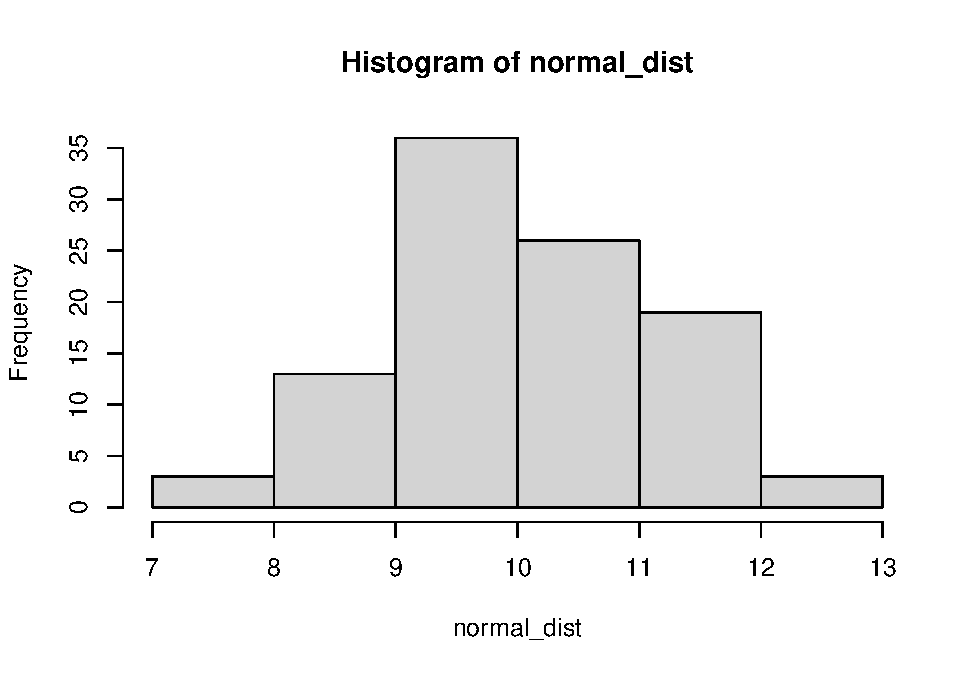
\includegraphics{_main_files/figure-latex/norm_dist_plot-1.pdf}

Another way to visualize this would be with a d

\hypertarget{what-is-normal}{%
\subsection{\texorpdfstring{What \emph{is} normal?}{What is normal?}}\label{what-is-normal}}

\hypertarget{quantitative-summaries}{%
\subsubsection{Quantitative summaries}\label{quantitative-summaries}}

5num summary
* Min, 25th percentile, median, 75th percentile, Max

\begin{Shaded}
\begin{Highlighting}[]
\NormalTok{tab\_normal\_dist }\OtherTok{\textless{}{-}} \FunctionTok{summary}\NormalTok{(normal\_dist)}
\end{Highlighting}
\end{Shaded}

We can print the table in R by calling its name.

\begin{Shaded}
\begin{Highlighting}[]
\NormalTok{tab\_normal\_dist}
\end{Highlighting}
\end{Shaded}

\begin{verbatim}
##    Min. 1st Qu.  Median    Mean 3rd Qu.    Max. 
##   6.987   9.448  10.035  10.012  10.735  13.033
\end{verbatim}

Mean, standard deviation

\hypertarget{meaningful-comparisons}{%
\subsubsection{Meaningful Comparisons}\label{meaningful-comparisons}}

How to compare apples to oranges? Standardize the units / standardize the data

\begin{Shaded}
\begin{Highlighting}[]
\NormalTok{data1 }\OtherTok{\textless{}{-}} \FunctionTok{rnorm}\NormalTok{(}\AttributeTok{n=}\DecValTok{1000}\NormalTok{, }
              \AttributeTok{mean =} \DecValTok{100}\NormalTok{,}
              \AttributeTok{sd =} \DecValTok{10}\NormalTok{)}

\NormalTok{data2 }\OtherTok{\textless{}{-}} \FunctionTok{rnorm}\NormalTok{(}\AttributeTok{n=}\DecValTok{1000}\NormalTok{,}
               \AttributeTok{mean =} \DecValTok{60}\NormalTok{, }
               \AttributeTok{sd =} \DecValTok{25}\NormalTok{)}
\end{Highlighting}
\end{Shaded}

Are these the same distribution?

Any issues??

\begin{Shaded}
\begin{Highlighting}[]
\FunctionTok{layout}\NormalTok{(}\FunctionTok{matrix}\NormalTok{(}\DecValTok{1}\SpecialCharTok{:}\DecValTok{2}\NormalTok{, }\AttributeTok{ncol =} \DecValTok{2}\NormalTok{))}
\FunctionTok{hist}\NormalTok{(data1)}
\FunctionTok{hist}\NormalTok{(data2)}
\end{Highlighting}
\end{Shaded}

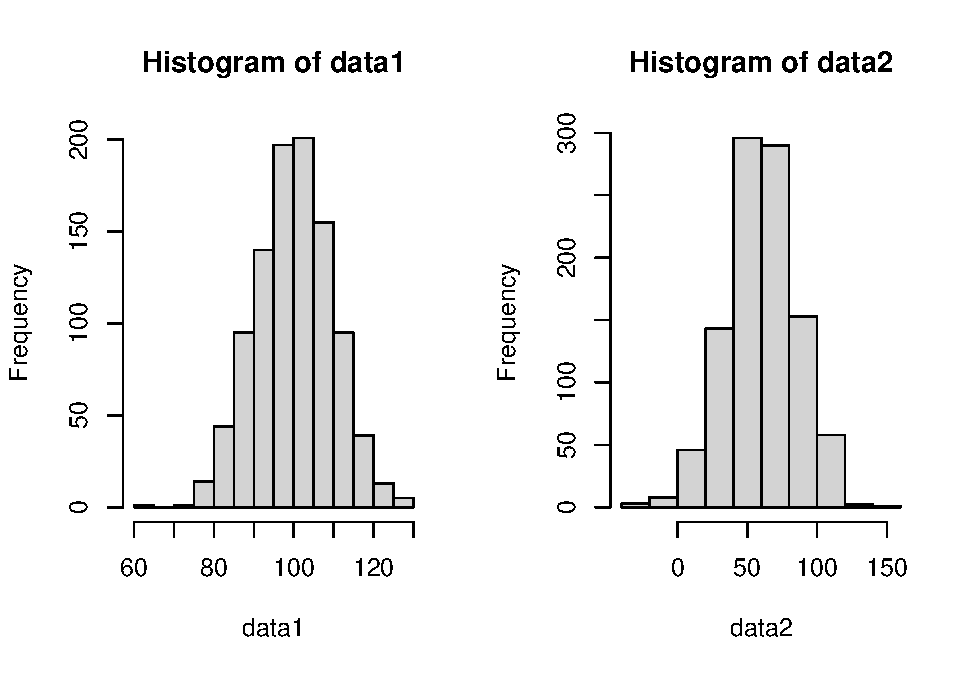
\includegraphics{_main_files/figure-latex/rnorm_hist_comp-1.pdf}

\begin{Shaded}
\begin{Highlighting}[]
\NormalTok{total\_range }\OtherTok{\textless{}{-}} \FunctionTok{range}\NormalTok{(data1, data2)}
\end{Highlighting}
\end{Shaded}

Are they the same?

\begin{Shaded}
\begin{Highlighting}[]
\FunctionTok{layout}\NormalTok{(}\FunctionTok{matrix}\NormalTok{(}\DecValTok{1}\SpecialCharTok{:}\DecValTok{2}\NormalTok{, }\AttributeTok{ncol =} \DecValTok{2}\NormalTok{))}
\FunctionTok{hist}\NormalTok{(data1, }\AttributeTok{xlim =}\NormalTok{ total\_range)}
\FunctionTok{hist}\NormalTok{(data2, }\AttributeTok{xlim =}\NormalTok{ total\_range)}
\end{Highlighting}
\end{Shaded}

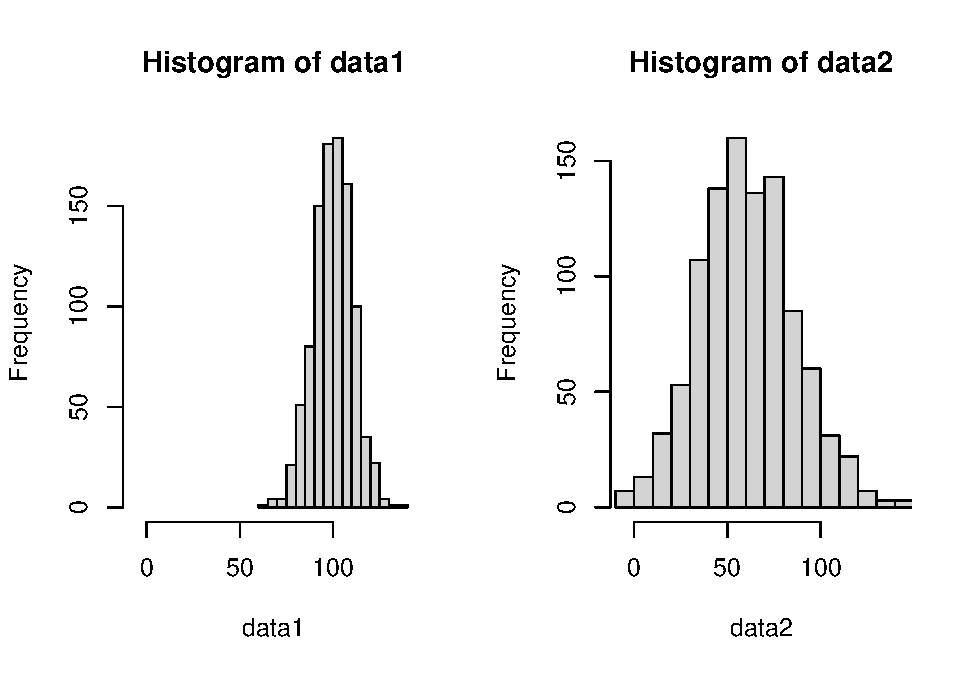
\includegraphics{_main_files/figure-latex/rnorm_hist_comp_true-1.pdf}

Numerically / tabularly

Often times its important to tables of \textbf{summary statistics}

\begin{Shaded}
\begin{Highlighting}[]
\NormalTok{norm\_comp\_tab }\OtherTok{\textless{}{-}} \FunctionTok{rbind}\NormalTok{(}\FunctionTok{summary}\NormalTok{(data1),}
                       \FunctionTok{summary}\NormalTok{(data2))}

\NormalTok{norm\_comp\_tab}
\end{Highlighting}
\end{Shaded}

\begin{verbatim}
##           Min.  1st Qu.    Median     Mean   3rd Qu.     Max.
## [1,]  71.26983 93.15937 100.10482 99.92318 106.51155 132.7447
## [2,] -14.53694 42.85820  60.91629 59.92596  77.18745 155.6257
\end{verbatim}

Making the table a little nicer. Also an example of \textbf{conditional programming}.

\begin{Shaded}
\begin{Highlighting}[]
\FunctionTok{rownames}\NormalTok{(norm\_comp\_tab) }\DocumentationTok{\#\# they\textquotesingle{}re null}
\end{Highlighting}
\end{Shaded}

\begin{verbatim}
## NULL
\end{verbatim}

\begin{Shaded}
\begin{Highlighting}[]
\ControlFlowTok{if}\NormalTok{(}\FunctionTok{is.null}\NormalTok{(}\FunctionTok{rownames}\NormalTok{(norm\_comp\_tab)))\{}
  \FunctionTok{rownames}\NormalTok{(norm\_comp\_tab) }\OtherTok{\textless{}{-}} \FunctionTok{c}\NormalTok{(}\StringTok{"data1"}\NormalTok{, }\StringTok{"data2"}\NormalTok{)}
\NormalTok{\}}
\end{Highlighting}
\end{Shaded}

When working with \textbf{Rmarkdown} we can take advantage of \texttt{knitr} and \texttt{pandoc} to nice looking tables even easier.

\begin{Shaded}
\begin{Highlighting}[]
\NormalTok{knitr}\SpecialCharTok{::}\FunctionTok{kable}\NormalTok{(norm\_comp\_tab)}
\end{Highlighting}
\end{Shaded}

\begin{tabular}{l|r|r|r|r|r|r}
\hline
  & Min. & 1st Qu. & Median & Mean & 3rd Qu. & Max.\\
\hline
data1 & 71.26983 & 93.15937 & 100.10482 & 99.92318 & 106.51155 & 132.7447\\
\hline
data2 & -14.53694 & 42.85820 & 60.91629 & 59.92596 & 77.18745 & 155.6257\\
\hline
\end{tabular}

\textbf{How} transform the data

Simple transformation (multiply all values by 100)
* to convert units
* other examples?

Complex transformations
* log-transformation (\emph{DEE: not a fan})
* z-scores (\emph{DEE: a better option})

\textbf{Why} transform the data?
* Real world applications?
* Is it always appropriate to transform data?

\hypertarget{skews}{%
\subsection{Skews}\label{skews}}

What to do if the data are \textbf{not} normal?

\hypertarget{week-3-statisitcal-testing-of-simple-data-sets-1}{%
\section{Week 3: Statisitcal testing of simple data sets}\label{week-3-statisitcal-testing-of-simple-data-sets-1}}

\hypertarget{t-tests-anova-chi2}{%
\subsection{t-tests, ANOVA, chi2}\label{t-tests-anova-chi2}}

\hypertarget{week-4-relationships-between-variables-in-simple-data-sets}{%
\section{Week 4: Relationships between variables in simple data sets}\label{week-4-relationships-between-variables-in-simple-data-sets}}

\hypertarget{correlation-linear-regression}{%
\subsection{Correlation, Linear Regression}\label{correlation-linear-regression}}

\hypertarget{simple-lm}{%
\subsubsection{Simple LM}\label{simple-lm}}

\hypertarget{complex-lm}{%
\subsubsection{Complex LM}\label{complex-lm}}

\hypertarget{genearlized-linear-model}{%
\subsection{Genearlized Linear Model}\label{genearlized-linear-model}}

\hypertarget{week-5}{%
\section{Week 5:}\label{week-5}}

For now, I have 3 main chapters for each of the main sections:
* Basics of data science / R \ref{unit1}
* Applications/critiques using IPUMS data \ref{unit2}
* Student-driven projects \ref{unit3}

Each of these \textbf{Chapters} contains multiple sections. We'll likely want to break these sections out into their own \texttt{.Rmd} files as they get fleshed out. For now, I'll try to keep the abundance of files limited.

\textbf{NOTE:} As these actually get filled out, we will probably want to insert different \texttt{part}s to the book (EG, the content of Unit 1 is covered in \texttt{Part\ I}).
* Declare parts with \texttt{\#\ (PART)\ Part\ I\ \{-\}} immediately before the first chapter \texttt{\#} it contains.

\textbf{Topics to include:}
* What is data?
* Everything can be data
* How do we interpret data
* Tables
* Plots
* Univariate distributions
* What can they tell us
* Multi-modality in distributions
* Categorical vs continuous data
* Don't need to get ahead of this yet
* Add in a grouping category - multi state/multi-national dataset
* Ttest / anova

\textbf{Type of Data:}
Age distributions
Specifically generate a dataset with old/young folks over-represented to highlight a bimodal distribution

Start with single state/country
Add a second state/country to demo ttest
Add more to demo anova

Alternatively, income by education level - may be more interesting/relevant to college students (or depressing)

\hypertarget{intro-to-rrstudio}{%
\section{Intro to R/RStudio}\label{intro-to-rrstudio}}

\hypertarget{reading-data-distributions}{%
\section{Reading Data / Distributions}\label{reading-data-distributions}}

\hypertarget{what-is-a-normal-distribution}{%
\subsection{\texorpdfstring{What \emph{is} a \textbf{normal distribution}}{What is a normal distribution}}\label{what-is-a-normal-distribution}}

\hypertarget{how-normal-is-it}{%
\subsubsection{How normal is it?}\label{how-normal-is-it}}

show increasingly unclear examples of normal vs not

introduce tests of normality

\hypertarget{measuring-normality---single-sample}{%
\subsubsection{Measuring normality - single sample}\label{measuring-normality---single-sample}}

reinforce {[}concept of statistical{]} \textbf{normality}

is a value from a sample? - one way ttest
something about tails

\hypertarget{comparing-normality---two-saples}{%
\subsubsection{comparing normality - two saples}\label{comparing-normality---two-saples}}

standard / two-way t test

\hypertarget{comparing-more-than-two---anova}{%
\subsubsection{comparing more than two - ANOVA}\label{comparing-more-than-two---anova}}

\hypertarget{unit2}{%
\chapter{IPUMS}\label{unit2}}

\hypertarget{week-6-exploratory-analysis-1}{%
\section{Week 6 Exploratory analysis}\label{week-6-exploratory-analysis-1}}

\hypertarget{week-7-hypothesis-testing-1}{%
\section{Week 7 Hypothesis Testing}\label{week-7-hypothesis-testing-1}}

\hypertarget{week-8-statistical-inference-1}{%
\section{Week 8 Statistical Inference}\label{week-8-statistical-inference-1}}

\hypertarget{week-9-tbd-1}{%
\section{Week 9 (TBD)}\label{week-9-tbd-1}}

\hypertarget{week-10-tbd-1}{%
\section{Week 10 (TBD)}\label{week-10-tbd-1}}

Some text to break up the sub-section headers

\hypertarget{intro-to-ipums-website}{%
\section{Intro to IPUMS website}\label{intro-to-ipums-website}}

\hypertarget{background-on-ipums}{%
\subsection{background on ipums}\label{background-on-ipums}}

\hypertarget{navigating-website}{%
\subsection{navigating website}\label{navigating-website}}

Find certain (very common) variables to answer (common) social science questions.

We describe our methods in this chapter.

Math can be added in body using usual syntax as follows. This may be useful, particularly for explaining the math side of things.

\hypertarget{math-example}{%
\section{math example}\label{math-example}}

\(p\) is unknown but expected to be around 1/3. Standard error will be approximated

\[
SE = \sqrt(\frac{p(1-p)}{n}) \approx \sqrt{\frac{1/3 (1 - 1/3)} {300}} = 0.027
\]

You can also use math in footnotes like this\footnote{where we mention \(p = \frac{a}{b}\)}. Footnotes are helpful because they re-link to where you left off.

We will approximate standard error to 0.027\footnote{\(p\) is unknown but expected to be around 1/3. Standard error will be approximated

  \[
  SE = \sqrt(\frac{p(1-p)}{n}) \approx \sqrt{\frac{1/3 (1 - 1/3)} {300}} = 0.027
  \]}

The \texttt{longnote} footnote seems particularly useful.

\hypertarget{unit3}{%
\chapter{Unit 3: Independent Research}\label{unit3}}

\hypertarget{week-11-students-develop-research-question-1}{%
\section{Week 11: Students develop research Question}\label{week-11-students-develop-research-question-1}}

\hypertarget{week-12-students-find-relevant-variables-from-ipums-1}{%
\section{Week 12: Students find relevant variables from IPUMS}\label{week-12-students-find-relevant-variables-from-ipums-1}}

\hypertarget{week-13-students-test-and-evaluate-results-1}{%
\section{Week 13: Students test and evaluate results}\label{week-13-students-test-and-evaluate-results-1}}

\hypertarget{week-14-students-prepare-presentations-of-results-1}{%
\section{Week 14: Students prepare presentations of results}\label{week-14-students-prepare-presentations-of-results-1}}

\hypertarget{week-15-students-present-work-slides-poster-podium-etc-1}{%
\section{Week 15: Students present work (slides, poster, podium, etc)}\label{week-15-students-present-work-slides-poster-podium-etc-1}}

By this point, students should be familiar with basic concepts from Chapter \ref{unit1}. These include:

\begin{itemize}
\tightlist
\item
  Basic Coding

  \begin{itemize}
  \tightlist
  \item
    read/write data in/out of R
  \item
    basic manipulations
  \end{itemize}
\item
  Theoretical Basis

  \begin{itemize}
  \tightlist
  \item
    looking at data distributions
  \item
    formal assessment of distributions
  \end{itemize}
\end{itemize}

Students will also be familiar with how these concepts are applied from Chapter \ref{unit2}. Hopefully students will be able to:

\begin{itemize}
\tightlist
\item
  Come up with a social science question they are interested in

  \begin{itemize}
  \tightlist
  \item
    Critically think about target variable(s) of interest. Any \emph{a priori} covariates? confounders?
  \item
    Acquire relevant data from IPUMS
  \item
    Analyze, Summarize, Visualize Data

    \begin{itemize}
    \tightlist
    \item
      scope and complexity at student/teach discretion
    \end{itemize}
  \item
    Present research to class

    \begin{itemize}
    \tightlist
    \item
      \textbf{potentially} critically discuss/evaluate each others work.
    \item
      \textbf{science is collaborative} everyone should be out to do their best work and represent the data as best we can. We all have conscious and unconscious biases, and the best way to confront them is share and receive (respectful) feedback.
    \end{itemize}
  \end{itemize}
\end{itemize}

During this Unit, we suggest giving ample class time for independent student research, peer-to-peer collaboration, and basic R/stats troubleshooting. This would also be a great time to model how to give respectful criticism by discussing recent research papers.
* We could maybe come up with 1-2 seed examples, with a few talking points

\hypertarget{example-one}{%
\section{Example one}\label{example-one}}

\hypertarget{example-two}{%
\section{Example two}\label{example-two}}

\hypertarget{ex_code}{%
\chapter{Example RMD code}\label{ex_code}}

For now, this chapter is a bit of a placeholder. I'm not sure what/how the \texttt{references.Rmd} file actually fits in to the code/construction (it looks automatic) so I want to keep that in place and need a section to note that.

I also want a more centralized reference point to put any example code I find helpful while working in R/bookdown. This section could get really unrully really fast, but oh well.

\hypertarget{core}{%
\section{Core}\label{core}}

\texttt{index.Rmd} is required and treated as file \texttt{00}. Chapters \emph{should} be numbered for ease of sorting but custom orders are possible by specifying filenames somewhere \textbf{in this file}

Remember each Rmd file contains one and only one chapter, and a chapter is defined by the first-level heading \texttt{\#}.
+ \textbf{IE} beyond the YAML header this file functions as a normal chapter since it starts with a top level header.
+ Note that \texttt{index.Rmd} has its own YMAL in addition to the various .yml files\ldots not sure exactly how these relate.

Reference a figure by its code chunk label with the \texttt{fig:} prefix, e.g., see Figure @ref(fig:norm\_dist\_plot). Similarly, you can reference tables generated from \texttt{knitr::kable()}, e.g., see Table @ref(tab:norm\_summary\_tab).
* Again, this prints an auto-generated numeral
* also leaving this in the context of the plots in Chapter \ref{unit2}

You can write citations, too. See \texttt{knitr::write\_bib()} for more on this. Quick example from demo/index (may not work without write\_bib() though): we are using the \textbf{bookdown} package \citep{R-bookdown} in this sample book, which was built on top of R Markdown and \textbf{knitr} \citep{xie2015}.
* If included, ``Refernces'' section gets added to each chapter.
* Not exactly sure where

Embed html renders (EG, fancy tables (IPUMS\_var\_desc), or any shiny app) with \texttt{webshot} R package and \texttt{phantomJS}.

\begin{Shaded}
\begin{Highlighting}[]
\FunctionTok{install.packages}\NormalTok{(}\StringTok{"webshot"}\NormalTok{)}
\NormalTok{webshot}\SpecialCharTok{::}\FunctionTok{install\_phantomjs}\NormalTok{()}
\end{Highlighting}
\end{Shaded}

\hypertarget{tips}{%
\section{Tips}\label{tips}}

*\textbf{Autonumber sections} Note the \texttt{\{-\}} used to indicate ``do not number this section'' eg: preface.

\textbf{LABEL EVERYTHING} you'll likely want to reference it later
* code chunks that produce figures can be referenced via \texttt{@\textbackslash{}ref(fig:{[}LABEL{]})}

You can label chapter and section titles using \texttt{\{\#label\}} after them, e.g., we can reference Chapter \ref{unit1}. If you do not manually label them, there will be automatic labels anyway,
* No idea how the automatic references work, so always be sure to declare them.
* \textbf{NOTE} these display as the relevant Chapter \texttt{numeral}.

\hypertarget{syntax}{%
\section{Syntax}\label{syntax}}

\emph{italics} or
\emph{italics} (can handle spaces)
\textbf{bold}
\texttt{code}
\(equations\)

\hypertarget{math}{%
\subsection{Math}\label{math}}

Randal Pruim features an extensive list of common math expression on their \href{https://rpruim.github.io/s341/S19/from-class/MathinRmd.html}{github page}. Here are some quick notes:

In-line equations can be written within \texttt{\$} and will be displayed right there: \(a^2 + b^2 = c^2\). In contrast, you can also add equation chunks by using \texttt{\$\$}

This can be coded in-line, \[\sum_{n=1}^{10} n^2\], but will result in a page break.

Alternatively, a more ``classic'' equation chunk:

\$\$
Plain text doesnt get spaces

how

very

odd

\$\$

To compile this example to PDF, you need XeLaTeX. You are recommended to install TinyTeX (which includes XeLaTeX): \url{https://yihui.name/tinytex/}.

  \bibliography{book.bib,packages.bib}

\end{document}
